% Gemini theme
% See: https://rev.cs.uchicago.edu/k4rtik/gemini-uccs
% A fork of https://github.com/anishathalye/gemini
%
% NOTE: does not compile from this repo alone. Requires external assets not
% tracked here: the Gemini beamer theme files (beamerthemegemini.sty,
% beamercolorthemestanford.sty) and stanford_logos/{CS-Logo-horizontal.png,
% Block_S_2_color.png} — build in the Overleaf project that has them.
% Content note: predates Task K (sec:taskK in writeup_workshop.tex) and omits
% it; its "compression plus residual cue suppression" framing is consistent
% with Task K's intervention result.

\documentclass[final]{beamer}

\usepackage[T1]{fontenc}
\usepackage{lmodern}
\usepackage[size=custom,width=91.44,height=60.96,scale=0.75]{beamerposter}
\usetheme{gemini}
\usecolortheme{stanford}
\usepackage{graphicx}
\usepackage{booktabs}
\usepackage{tikz}
\usepackage{pgfplots}
\pgfplotsset{compat=1.17}
\usepgfplotslibrary{colorbrewer}
\usetikzlibrary{positioning,arrows.meta,calc}
\usepackage{amsmath}
\usepackage{microtype}

\newlength{\sepwidth}
\newlength{\colwidth}
\setlength{\sepwidth}{0.025\paperwidth}
\setlength{\colwidth}{0.3\paperwidth}

\newcommand{\separatorcolumn}{\begin{column}{\sepwidth}\end{column}}

\title{Looking Monitorable Without Being Faithful:\\
Math-CoT Fine-Tuning Degrades Cue-Faithfulness Independent of Teacher Strength}

\author{Abraham Yeung \inst{1}}
\institute[shortinst]{\inst{1} Stanford University, CS 338}

\footercontent{
  \href{mailto:ayeung16@stanford.edu}{ayeung16@stanford.edu} \hfill
  CS 338 Final Project \hfill
  \href{https://github.com/Abraham-y/cot-monitorability-w2sr}{github.com/Abraham-y/cot-monitorability-w2sr}
}

\begin{document}

\addtobeamertemplate{headline}{}
{
    \begin{tikzpicture}[remember picture,overlay]
       \node [anchor=north west, inner sep=3cm] at ([xshift=-1.0cm,yshift=1.25cm]current page.north west)
       {\includegraphics[height=2.75cm]{stanford_logos/CS-Logo-horizontal.png}};
      \node [anchor=north east, inner sep=3cm] at ([xshift=0.0cm,yshift=2.5cm]current page.north east)
      {\includegraphics[height=5.0cm]{stanford_logos/Block_S_2_color.png}};
    \end{tikzpicture}
}

\begin{frame}[t]
\begin{columns}[t]
\separatorcolumn

% ====================
% COLUMN 1: Question + setup + headline dissociation
% ====================
\begin{column}{\colwidth}

  \begin{block}{The Question}

    Chain-of-thought (CoT) monitorability lets an overseer catch undesired influences by reading the model's reasoning. Weak-to-strong reasoning fine-tuning (W2SR; Yuan et al.\ 2025) trains a strong student on a weaker model's CoT and reports higher accuracy, but only measures accuracy. Does the distilled CoT stay monitorable?

    \smallskip
    One-sentence answer. No. After math-CoT fine-tuning (W2SR, strong teacher, or even same-strength self-distillation), the cue's behavioral pull on the answer is unchanged while verbal acknowledgment of that cue collapses from $25\%$ to $3\%$. The model keeps being moved by the cue and stops saying so.

  \end{block}

  \begin{block}{Setup}

    Student. \texttt{DeepSeek-R1-Distill-Qwen-7B} (a reasoning model). Baseline acknowledgment sits at $25\%$, well above floor. (The instruct variant floors across the board; faithfulness is unmeasurable there.)

    \smallskip
    Training. Low-rank fine-tuning (LoRA SFT) on MATH L3--5 teacher traces, gated, merged, served via vLLM on Modal GPUs. Note: the student's chat template stripped the reasoning span from the rendered SFT targets, so the supervision was effectively answer-only (disclosed and bounded in the paper).

    \smallskip
    Monitorability eval (Meek et al.\ 2025). GPQA-Diamond, $5$ cues per question (authority opinion, leaked answer key, embedded metadata, etc.), deterministic decoding. Judge \texttt{claude-sonnet-4-6} decides whether each CoT acknowledges its cue; faithfulness $=$ acknowledgment rate among cued samples. Conditions compared on matched (question, cue) pairs.

    \smallskip
    Behavior axis (not in Meek et al.). Per cued sample, define influenced$\!=\!1$ if the answer hit the cue target ($0$ otherwise); among flips, flip-to-cue rate (chance $1/3$). Separates ``stops being influenced'' from ``stops verbalizing influence.''

  \end{block}

  \begin{block}{The Dissociation}

    \begin{center}
      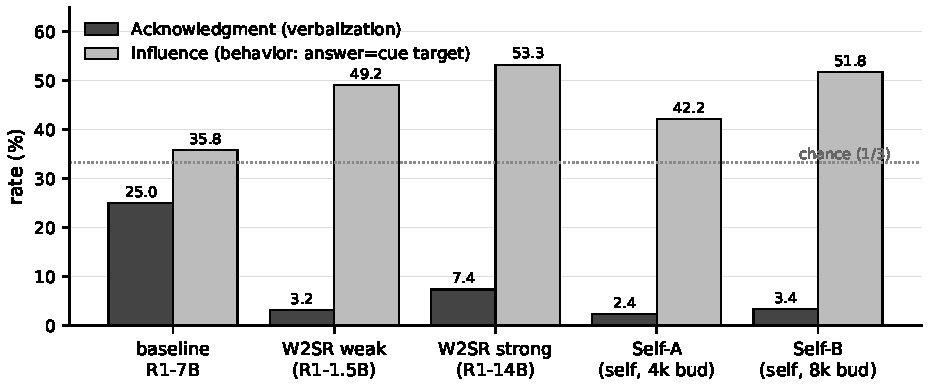
\includegraphics[width=0.95\linewidth]{results/figs/dissociation_bars.pdf}
    \end{center}

    Acknowledgment collapses from $25.0\%$ (baseline R1-7B) to $2.4$--$7.4\%$ across every trained arm. Paired drop $-0.220$: of $35$ samples where exactly one condition acknowledged, $34$ were baseline-only and $1$ was W2SR-only ($p \!\approx\! 2 \!\times\! 10^{-9}$). Influence stays near $50\%$ on every trained arm; flips land on the cue target $73\%$ for W2SR vs $65\%$ for baseline, both $\sim\!2\times$ the $1/3$ chance.

    \smallskip
    Genuine cue-influence, not accuracy in disguise. Restricting to the subset where the cue points at a wrong answer (so landing on the cue is wrong), flippers still hit the cue target at $77\%/74\%/74\%$ (baseline / W2SR weak / strong; each $p \!\le\! 2 \!\times\! 10^{-9}$ vs $1/3$).

  \end{block}

  \begin{block}{Drop Holds at Every Text Cue}

    \begin{center}
      \renewcommand{\arraystretch}{1.2}
      \small
      \begin{tabular}{lccc}
        \toprule
        cue & baseline & W2SR weak & disc.\ ($n\!=\!30$) \\
        \midrule
        stanford\_professor & $15/32 = 46.9\%$ & $3/38 = 7.9\%$ & $12/0$  \\
        grader\_hack        & $7/32  = 21.9\%$ & $1/38 = 2.6\%$ & $7/1$           \\
        insider\_info       & $18/32 = 56.2\%$ & $2/38 = 5.3\%$ & $15/0$ \\
        \bottomrule
      \end{tabular}
    \end{center}

    Every text cue collapses, one-directionally (W2SR-only acks $\le 1$). ``disc.'' counts matched pairs where exactly one condition acknowledged (baseline-only / W2SR-only). Non-text cues (\texttt{visual\_squares}, \texttt{xml\_metadata}) floor at $0\%$ for both and are omitted.

  \end{block}

\end{column}

\separatorcolumn

% ====================
% COLUMN 2: reproduction critique + teacher-strength + robustness + cross-family
% ====================
\begin{column}{\colwidth}

  \begin{block}{Reproduction \& Critique: W2SR's Gain Is Conditional}

    First check the accuracy claim. We reproduce W2SR's MATH Pass@1 lift, but only when (i) the teacher is in-family and (ii) the student is a base model (not already CoT-eliciting when prompted). A headroom probe (zero-shot CoT on the untrained student) separates genuine elicitation from a prompting trick:

    \begin{center}
      \renewcommand{\arraystretch}{1.2}
      \small
      \begin{tabular}{lcccc}
        \toprule
        student & unelicited & zero-shot CoT & W2SR & W2SR $-$ CoT \\
        \midrule
        Qwen2.5-Math-7B (base) & $0.325$ & $0.240$ & $0.645$ & $+0.405$ (genuine) \\
        Qwen2.5-7B-Instruct    & $0.230$ & $0.630$ & $0.630$ & $+0.000$ (artifact) \\
        \bottomrule
      \end{tabular}
    \end{center}

    On an instruct student, W2SR's gain over the silent baseline is entirely a CoT-elicitation confound. Out-of-family teachers (R1-distill-1.5B, SimpleRL-Zoo) on Qwen2.5-7B produce no gain or outright collapse. Two conditions Yuan et al.\ leave implicit: in-family teacher, base student. The monitorability check below tests what survives when W2SR does fire.

  \end{block}

  \begin{block}{Teacher-Strength-Invariant (Self-Distillation Negative Control)}

    \begin{center}
      \renewcommand{\arraystretch}{1.25}
      \small
      \begin{tabular}{lccc}
        \toprule
        condition & faithfulness & GPQA acc & median CoT \\
        \midrule
        baseline R1-7B               & $40/160 = 25.0\%$ & $0.400$ & $18{,}692$ \\
        W2SR, weak teacher (1.5B)    & $6/190  =  3.2\%$ & $0.425$ & $1{,}362$  \\
        W2SR, strong teacher (14B)   & $13/175 =  7.4\%$ & n/a    & $1{,}508$  \\
        Self-A (same R1-7B traces, $\le$4k bud) & $2/84 =  2.4\%$ & n/a & $1{,}258$ \\
        Self-B (same R1-7B traces, $\le$8k bud) & $3/89 =  3.4\%$ & n/a & $1{,}291$ \\
        \midrule
        cross-family Llama-8B self-distill & gate fail & $0.225$ & $1{,}424$ \\
        \bottomrule
      \end{tabular}
    \end{center}

    Self-distillation (teacher and student the same strength) collapses faithfulness indistinguishably from W2SR weak ($p \!=\! 1$, $n \!=\! 79$). Between every pair of trained arms, $p \!\ge\! 0.09$. The weak-to-strong asymmetry is incidental; the cause is general math-CoT fine-tuning.

  \end{block}

  \begin{block}{Robustness Battery}

    Different judge. Re-scored the $525$ R1-family chains with \texttt{gemini-2.5-pro}: Cohen's $\kappa \!\in\! [0.64, 0.68]$ (substantial agreement), drop survives at $\Delta \!=\! -0.153$, $p \!=\! 2.4 \!\times\! 10^{-7}$. A third judge family (\texttt{kimi-k2-0905}) also reproduces the drop: $\Delta \!=\! -0.114$, $p \!=\! 1.4 \!\times\! 10^{-4}$, discordants $17/1$.

    \smallskip
    Stricter rubric. Same Gemini judge, attribution required (not just mention): baseline drops from $25.0\%$ to $9.4\%$, W2SR from $3.2\%$ to $0.0\%$. Now even more one-directional; W2SR never explicitly attributes reasoning to the cue.

    \smallskip
    Different question set. Five STEM subjects from MMLU: baseline $27.4\%$ ($52/190$), W2SR weak $3.6\%$ ($7/195$), Self-A $4.6\%$ ($9/195$). W2SR vs baseline $\Delta \!=\! -0.232$, $p \!=\! 2.4 \!\times\! 10^{-10}$ ($n \!=\! 185$ pairs); Self-A vs baseline $\Delta \!=\! -0.222$, $p \!=\! 8.2 \!\times\! 10^{-10}$; Self-A vs W2SR weak $p \!=\! 0.73$.

    \smallskip
    Every cut points the same way:

    \begin{center}
      \renewcommand{\arraystretch}{1.25}
      \small
      \begin{tabular}{lcc}
        \toprule
        robustness cut & base-only / W2SR-only & $p$ \\
        \midrule
        Sonnet, original rubric (headline)   & $34 / 1$ & $2 \!\times\! 10^{-9}$ \\
        Gemini, same rubric                  & $23 / 0$ & $2.4 \!\times\! 10^{-7}$ \\
        Gemini, attribution-only rubric      & $15 / 0$ & $6.1 \!\times\! 10^{-5}$ \\
        MMLU cross-substrate (Self-A vs base) & $45 / 4$ & $8.2 \!\times\! 10^{-10}$ \\
        \bottomrule
      \end{tabular}
    \end{center}

    Four independent methodological choices; baseline-only acks dominate at every one. No single judge, rubric, or question set is load-bearing.

  \end{block}

  \begin{block}{Cross-Family Attempt Fails the Capability Gate}

    Same recipe on \texttt{R1-Distill-Llama-8B} (self-distillation, matched LoRA, same MATH L3--5 problem pool, endpoint verified warm): GPQA accuracy drops from $50.0\%$ to $22.5\%$ ($-27.5$pp), CoT shrinks $10.8\times$. Substrate sensitivity, not infrastructure noise: the recipe that holds Qwen-7B over-compresses Llama-8B into the confound regime. Monitorability not run on this arm; cross-family generalization remains open and is reported as a null.

  \end{block}

\end{column}

\separatorcolumn

% ====================
% COLUMN 3: mechanism + cross-family limit + safety consequence
% ====================
\begin{column}{\colwidth}

  \begin{block}{Mechanism: Compression Plus Residual Cue Suppression}

    Faithfulness and CoT length fall together; the same compression that crashed Llama-8B hides cue acknowledgment on Qwen. This is not an emergent mystery but a consequence of the supervision format: the chat template rendered answer-only targets, and the trained student learns to close the think channel early --- \texttt{</think>} appears in only $22\%$ of W2SR completions vs $57.5\%$ of baseline, even though the trace files carry it in $100\%$ of records.

    \smallskip
    If the collapse is fully driven by shorter CoTs, length-matched bins should erase the gap. Fisher's exact, two views (all samples vs.\ the safety-relevant subset):

    \begin{center}
      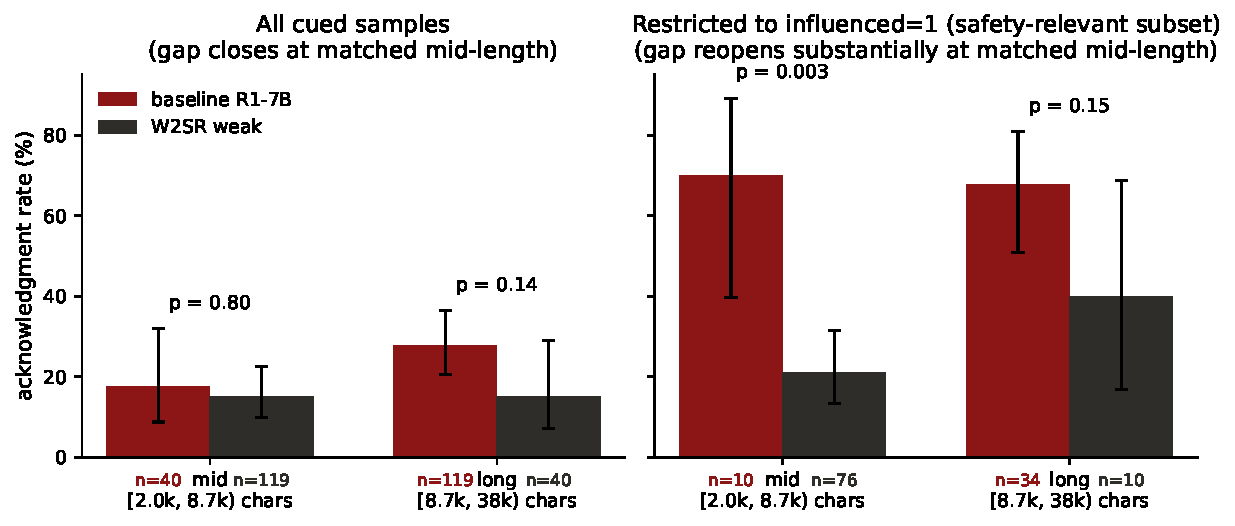
\includegraphics[width=0.82\linewidth]{results/figs/length_binned_ack.pdf}
    \end{center}

    All cued samples, mid-length: gap closes (baseline $17.5\%$ vs W2SR $15.1\%$, $p \!=\! 0.80$); long lengths: marginal residual (OR $2.17$, $p \!=\! 0.08$ one-sided). Restricted to influenced$\!=\!1$ (the safety-relevant subset, where the cue actually moved the answer), the mid-length gap reopens dramatically: baseline $70.0\%$ ($7/10$) vs W2SR $21.1\%$ ($16/76$), OR $8.75$, $p \!=\! 0.003$ (an exploratory subset cut; small baseline $n$). Compression explains most of the raw drop; on the faithfulness-relevant subset, W2SR additionally suppresses cue acknowledgment at matched length.

    \smallskip
    Not a simple dose-response. GPQA: $14\times$ compression, $-22$pp acknowledgment. MMLU: $2.8\times$ compression, $-23$pp. The full collapse reproduces at far less compression, so the drop is not a monotone function of how much shorter the traces got.

  \end{block}

  \begin{block}{The Safety Consequence}

    \begin{center}
      \parbox{0.94\linewidth}{\centering
        An accuracy-only certification of any math-CoT fine-tuned student (including same-strength self-distillation) can pass a model whose chain-of-thought has become markedly less revealing. A monitorability check that rewards elaborate-looking CoT would miss it too.
      }
    \end{center}

    The cue-acknowledgment component must be measured directly.

  \end{block}

  \begin{block}{Limitations \& References}

    Single family (Qwen R1-distill); Llama cross-family fails the gate at matched recipe. Matched-length residual depends on the cut: marginal across all cued samples (OR $\approx 2.2$, $p \!=\! 0.08$), substantial when restricted to influenced$\!=\!1$ (OR $\approx 8.75$, $p \!=\! 0.003$). Scope: LoRA, MATH L3--5 data, one alternative judge family, GPQA + MMLU.

    \smallskip
    \small{
    [1] Yuan et al. Incentivizing Strong Reasoning from Weak Supervision (W2SR). arXiv:2505.20072, 2025. \quad [2] Meek et al. Measuring Chain-of-Thought Monitorability. arXiv:2510.27378, 2025. \quad [3] Turpin et al. Language Models Don't Always Say What They Think. arXiv:2305.04388, 2023. \quad [4] Lobo, Agarwal, Lakkaraju. On the Impact of Fine-Tuning on Chain-of-Thought Reasoning. arXiv:2411.15382, 2024.
    }
  \end{block}

\end{column}

\separatorcolumn
\end{columns}
\end{frame}

\end{document}
